\chapter{A Program in a Web Page}\label{ch-web}

Everything so far has run in a terminal or on a board. Version 0.2 of
Zeno adds one more place: a web page. A button, a box to type in and a
list are written in HTML, as any page is, and what they \emph{do} is
written in Zeno. \verb|zeno build --web| puts the two into one file
that any browser opens.

\section{A first page}

A page that counts presses of a button. The page itself is plain HTML,
with no script in it:

\begin{zeno}[file=count.html, dir=count, run=no]
<!doctype html>
<html>
<body>
<button id="press">Press me</button>
<p id="count"></p>
</body>
</html>
\end{zeno}

And this is what it does:

\begin{zeno}[file=count.zeno, dir=count]
import web

let button = web.element("#press")
let count = web.element("#count")
var presses = 0

button.on("click", function() {
    presses += 1
    count.text = f"{presses} presses"
})

count.text = "no presses yet"
\end{zeno}

\verb|web.element("#press")| finds the element whose \verb|id| is
\verb|press|. \verb|button.on("click", ...)| gives the button a
function to call each time it is pressed, and \verb|count.text = ...|
changes what a paragraph shows.

The program was run here by \verb|zeno run|, which has no browser. It
runs the program on a \emph{simulated page}, which prints a line for
each change that somebody looking at the page would see. Nobody
presses a button on a simulated page, so it shows only what the
program did as it started. To see it in a browser, build it:

\begin{zeno}[file=count.zeno, dir=count, show=no, cmd=zeno build --web {file}]
import web

let button = web.element("#press")
let count = web.element("#count")
var presses = 0

button.on("click", function() {
    presses += 1
    count.text = f"{presses} presses"
})

count.text = "no presses yet"
\end{zeno}

\verb|zeno build --web count.zeno| looked for \verb|count.html| beside
the program, and wrote \verb|count.web.html|: the page, with the
program inside it. Open that file in a browser, from the disk, and the
button counts. It is one file and needs nothing else, so it can also
be mailed, or put on any web server as it is.

\section{The web module}

\verb|import web| brings in five functions:

\begin{center}
\begin{tabular}{lP{8.4cm}}
\toprule
Function & What it does \\
\midrule
\verb|web.element(selector)| & the first element that answers to the
  selector. Stops the program if the page has none \\
\verb|web.elements(selector)| & every element that answers to it, as a
  list, which may be empty \\
\verb|web.create(tag, text)| & a new element with that text in it, not
  on the page until it is appended to one that is \\
\verb|web.after(time, f)| & call \verb|f| once, that much later. The
  time has a unit: \verb|web.after(500 ms, tick)| \\
\verb|web.on_key(f)| & call \verb|f| with the name of each key that is
  pressed: \verb|"a"|, \verb|"Enter"|, \verb|"ArrowLeft"| \\
\bottomrule
\end{tabular}
\end{center}

A \emph{selector} is what CSS calls one. \verb|#count| is the element
with that \verb|id|, \verb|.done| every element of that class,
\verb|li| every list item, and \verb|#list li.done| every done item
inside the list.

What these give is an \verb|Element|, a type like any other: a
function can ask for one and a list can hold them. It has two fields
and eleven methods:

\begin{center}
\begin{tabular}{lP{8.4cm}}
\toprule
On an element & What it does \\
\midrule
\verb|e.text| & the text in it; give it a new value to change what the
  page shows \\
\verb|e.value| & what has been typed into it, for a box \\
\verb|e.on(event, f)| & call \verb|f| whenever that happens to it:
  \verb|"click"|, \verb|"input"|, \verb|"submit"|, or any event a
  browser has \\
\verb|e.append(child)| & \verb|child| becomes the last thing inside it \\
\verb|e.remove()| & it leaves the page \\
\verb|e.clear()| & everything inside it leaves the page \\
\verb|e.add_class(c)|, \verb|e.remove_class(c)| & give it a class, or
  take one away \\
\verb|e.has_class(c)| & whether it has that class \\
\verb|e.show()|, \verb|e.hide()| & whether it is shown at all \\
\verb|e.get(name)|, \verb|e.set(name, v)| & an attribute, such as
  \verb|href|. \verb|get| gives \verb|none| for one it does not have \\
\bottomrule
\end{tabular}
\end{center}

How a thing looks is the page's business, written in CSS. A program
changes the look by giving an element a class, and the CSS says what
that class looks like.

\begin{zeno}
import web

let note = web.element("#note")
let link = web.element("#help")
note.add_class("warning")
note.hide()
link.set("href", "/help")
print(link.get("href"), link.get("title"))
\end{zeno}

\section{A function the page calls takes nothing}

A function given to \verb|on| or \verb|after| is called by the page,
later, with nothing. There is no event object to unpack. The function
already knows which element it is for, because it was written where
that element was in reach:

\begin{zeno}[fails=yes]
import web

let button = web.element("#press")
button.on("click", function(event: int) {
    print(event)
})
\end{zeno}

The one thing an event carries that a program cannot find out another
way is which key was pressed, so \verb|web.on_key| is the one function
that hands something over: the key's name, as a \verb|str|.

\begin{why}
An event object in a browser has dozens of fields, and nearly every
handler reads none of them. A function that takes nothing has one way
to be written, and needs no type that a beginner must look up. The
element is in reach by the closure, as \hyperref[ch-function-values]{Functions
as Values} showed. (Decision 14.5.)
\end{why}

\section{A list of things to do}

The \verb|examples| folder has a page that is a whole small program: a
list of things to do. You type one and press Enter, and it joins the
list; a click marks it done, and another click takes that back. The
page is a form, an empty list, and a line that says how much is left:

\begin{zeno}[src=examples/todo.html, file=todo.html, dir=todo, run=no]
\end{zeno}

The program is the rest. Each thing gets its own function for its
clicks, written inside \verb|add| where the new \verb|item| is in
reach:

\begin{zeno}[src=examples/todo.zeno, file=todo.zeno, dir=todo, cmd=zeno run {file}]
\end{zeno}

Built with \verb|zeno build --web todo.zeno| and opened in a browser,
after typing two more things and clicking one:

\begin{center}
{\setlength{\fboxsep}{0pt}\fbox{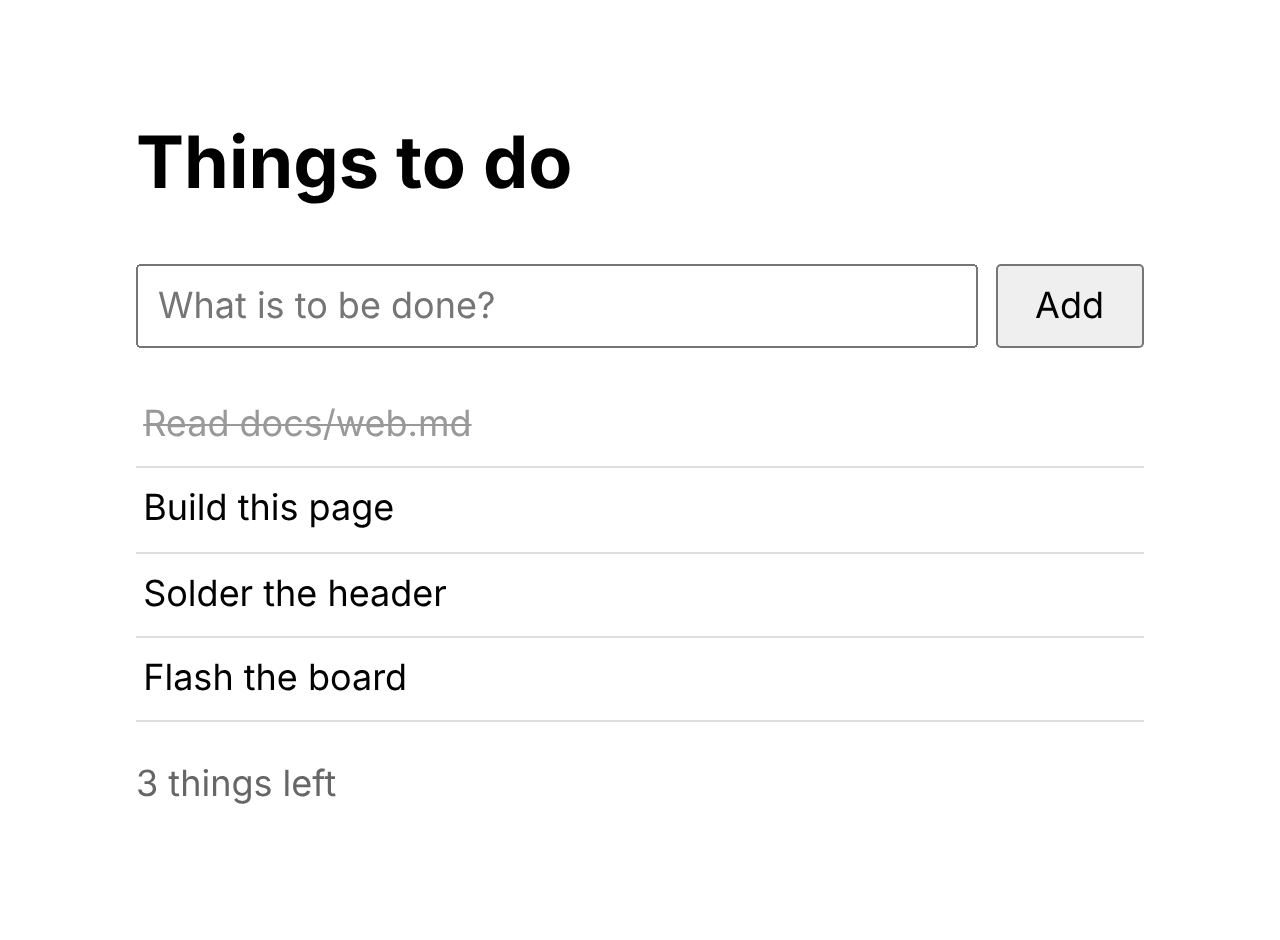
\includegraphics[width=0.7\textwidth]{images/todo.png}}}
\end{center}

\section{Testing a page}

The simulated page is not only for running. Because no button is ever
pressed on it, the tests press them, by calling the functions the page
would call. The two tests at the end of \verb|todo.zeno| do exactly
that: one adds a thing, and one sends the form with only spaces in the
box. \verb|zeno test| runs them with no browser:

\begin{zeno}[src=examples/todo.zeno, file=todo.zeno, dir=todo, show=no, cmd=zeno test {file}]
\end{zeno}

So what a page does can be tested in the same run as every other test,
by the same engines, as \hyperref[ch-testing]{Testing} showed.

There are two things the simulated page cannot tell you. It has no
HTML to look in, so it has every element that is asked for: a
misspelled \verb|web.element("#cuont")| works on a desk and stops the
program in the browser, with a message naming the selector. And it
reads only plain selectors: a tag, \verb|.class| and \verb|#id|,
together (\verb|li.done|) and one inside another (\verb|#list li|).
For any other it stops, rather than pretend the page has nothing:

\begin{zeno}[fails=yes]
import web

for item in web.elements("ul > li") {
    print(item.text)
}
\end{zeno}

The page that is built can use any selector a browser reads.

\section{A program with no page}

\verb|zeno build --web| needs no HTML of yours. With no page beside
the program, it writes one that shows what the program prints, so any
program that runs under \verb|zeno run| and reads no file can be put
in a page:

\begin{zeno}[file=hello.zeno, dir=hello, cmd=zeno build --web {file}]
for n in range(1, 4) {
    print(f"{n} squared is {n * n}")
}
\end{zeno}

In a page of your own, \verb|print| goes to the browser's console, and
also into the element with the id \verb|zeno-output| if the page has
one: put \verb|<pre id="zeno-output"></pre>| in the page to see it.

An error that nothing catches stops the program, as it does under
\verb|zeno run|, and is shown in a box at the foot of the page with its
line and column. After that the page calls nothing more, because a
program that went wrong halfway through a function has variables that
are half changed.

\section{How it works}

A browser runs two kinds of program: JavaScript, and
\emph{WebAssembly}, a small instruction set that a compiler can aim at
as it aims at a processor. Rust is one such compiler. So
\verb|zeno.wasm| is the Zeno you already have, the lexer, the parser,
the checker and the interpreter, compiled for a browser in place of a
desk. Nothing of Zeno was written again for it, and that is why a
program means the same in a page as under \verb|zeno run|: the same
checker checks it, and the same interpreter runs it.

A built page holds three things: the program as you wrote it,
\verb|zeno.wasm| written out as text, and a short piece of JavaScript
that starts the one with the other. WebAssembly can only do arithmetic
and call functions, and only numbers cross between it and the page.
So text crosses as a place in memory and a length, an element as a
number that the JavaScript looks up in a table, and every request to
the page, such as "set the text of element 4", as one line of JSON
through a single function. However many things the \verb|web| module
learns to do, the line between Zeno and the browser stays five
functions wide.

\verb|zeno build --web| finds \verb|zeno.wasm| where the variable
\verb|ZENO_WASM| says, or else beside \verb|zeno| itself, which is
where a release puts it (\hyperref[ch-getting-zeno]{Getting Zeno}).

\section{What a page cannot do}

\begin{description}
\item[Wait.] A browser has one thread for a page, and a program that
  sleeps on it stops the page drawing and the buttons working. In a
  page, \verb|time.sleep| is an error that says to use
  \verb|web.after(500 ms, ...)|, which lets the page go on in between.
\item[Go very deep.] The interpreter calls itself for each nested call
  of the program, on the browser's stack, which is small. Zeno counts,
  and stops at 200 nested calls in a page, with its own message, where
  on a desk the limit is 1000.
\item[Be built as firmware.] \verb|--firmware|, \verb|--no-collector|,
  \verb|--llvm| and \verb|--memory| are for a compiled program, and
  are refused with \verb|--web|. A page runs the interpreter.
\end{description}

And some things the \verb|web| module does not have yet: the style of
one element (use a class), where the mouse is, drawing, the network,
and anything kept between visits. Every built page carries the whole
of \verb|zeno.wasm|, about one and a half megabytes as text, and runs
at the speed of \verb|zeno run|: plenty for a page that waits for
clicks, and not enough for a game that draws sixty times a second. The
program is in the page as it was written, comments and all, for anyone
who opens the page to read.

\begin{why}
A page could have been made by compiling Zeno to JavaScript, or
through C or LLVM to WebAssembly. Each of those is one more engine to
hold to the same answers as the others, and JavaScript has no 64-bit
whole number to be an \verb|int|. Compiled Zeno is also strict Zeno,
so a page would have had a smaller language than a desk. Running the
interpreter itself in the browser adds no engine, and the whole
language is there on the first day. A small, fast page compiled
through C or LLVM is still open, and the \verb|web| module would not
change for it. (Decision 14.1.)
\end{why}

\begin{summary}
\verb|import web| finds elements with \verb|web.element| and
\verb|web.elements|, makes them with \verb|web.create|, and calls a
function later with \verb|web.after| or on a key with
\verb|web.on_key|. An \verb|Element| has \verb|text| and \verb|value|,
and methods to listen, append, remove, and change classes and
attributes. A function the page calls takes nothing.
\verb|zeno build --web| joins \verb|name.html| and \verb|name.zeno|
into one \verb|name.web.html|. Under \verb|zeno run| and
\verb|zeno test| the page is simulated, so a page can be tested
without a browser.
\end{summary}

\begin{tryit}
\begin{enumerate}
\item Build \verb|count.zeno| and open it. Then add a second button
  that sets the count back to zero.
\item Spell \verb|#list| wrong in \verb|todo.zeno|. What does
  \verb|zeno run| say, and what does the page say?
\item Add a button to \verb|todo.html| that removes every thing that is
  done. You need \verb|web.elements(".done")|. Write the test first.
\item Make a clock: a paragraph that shows how many seconds the page
  has been open, with a function that sets the text and then asks
  \verb|web.after(1 s, ...)| to call itself again.
\item Use \verb|web.on_key| to move a mark left and right along a line
  of text with the arrow keys.
\end{enumerate}
\end{tryit}
